\chapter{\IfLanguageName{dutch}{Long list}{Long list}} \label{chap:Long list}%
\label{ch:long-list}

\section{\IfLanguageName{dutch}{Spraakherkening}{Speech recognition}}\label{sec:Speech recognition}%

\subsection{Google Cloud Speech-to-text API}%

\paragraph{\IfLanguageName{dutch}{Beschrijving}{Description}}
Google Cloud Speech-to-text API is Google's kijk op spraakherkennigssoftware. De API is heel betrouwbaar. Zo heeft het volgens \textcite{Anggraini2018} een succespercentage van 100\% voor normale stemmen en een percentage tussen 83,3\% en 90\% voor mensen met een spraakbeperking. Daarnaast bied het ook de mogelijkheid om het model uit te breiden door het nieuwe vocabulaire aan te leren.

\paragraph{\IfLanguageName{dutch}{Functies}{Features}}
De service komt met verschillende functies. Dit zijn de belangrijke kenmerken die ze adverteren:

\begin{itemize}
    \item \textbf{Taalherkenning}: De API ondersteunt spraakherkenning in verschillende talen en dialecten, waardoor gebruikers wereldwijd toegang hebben tot de dienst. Het kan automatisch de gesproken taal detecteren zonder voorafgaande taalconfiguratie.

    \item \textbf{Real-time streaming}: De API ondersteunt real-time streaming van spraak naar tekst, waardoor ontwikkelaars toepassingen kunnen bouwen die directe feedback en interactie vereisen, zoals live ondertiteling, spraakgestuurde commando's en real-time transcriberen.

    \item \textbf{Hoge nauwkeurigheid}: Dankzij de geavanceerde neurale netwerkmodellen levert de Speech-to-Text API nauwkeurige transcripties, zelfs in omgevingen met achtergrondgeluiden, verschillende spreekstijlen en spraak van meerdere sprekers.

    \item \textbf{Aanpasbare modellen}: Gebruikers kunnen de spraakherkenning aanpassen aan specifieke woordenschat en domeinen door aangepaste woordenlijsten en grammatica's te gebruiken. Dit verhoogt de nauwkeurigheid en zorgt voor een betere herkenning van vakspecifieke terminologie.

    \item \textbf{Multimediaondersteuning}: De API kan spraak herkennen in verschillende formaten, waaronder audio-opnamen, audiobestanden en streaming-audio. Dit maakt integratie met verschillende bronnen en toepassingen mogelijk.

    \item \textbf{Beveiliging en privacy}: Google Cloud hanteert strenge beveiligingsmaatregelen om de vertrouwelijkheid en integriteit van de gegevens te waarborgen. De API ondersteunt ook automatische verwijdering van persoonlijk identificeerbare informatie (PII) uit de gegenereerde transcripties.

    \item \textbf{Spraakherkenning op apparaat}: Naast de cloudgebaseerde API biedt Google Cloud ook een on-device spraakherkenning SDK aan, genaamd Speech-to-Text On-Device. Hiermee kunnen ontwikkelaars spraakherkenning rechtstreeks op apparaten uitvoeren, zonder een internetverbinding te vereisen.
\end{itemize}

\paragraph{\IfLanguageName{dutch}{Tarieven}{Pricing}}
De service kan per maand 60 minuten gratis gebruikt worden. Daarna moet er betaald worden per minuut van €0,016 voor standaard met datalogging tot €0,072 voor medisch gebruik zonder datalogging.

\subsection{Amazon Transcribe}%

\paragraph{\IfLanguageName{dutch}{Beschrijving}{Description}}
Amazon Web Services (AWS) bied een ASR software aan genaamd Amazon Transcribe.

\paragraph{\IfLanguageName{dutch}{Functies}{Features}}
De functies die Amazon Transcribe aanbied zijn:

\begin{itemize}
    \item \textbf{Taalherkenning}: Amazon Transcribe kan automatisch de gesproken taal detecteren, waardoor het mogelijk is om meertalige spraakherkenning te realiseren zonder voorafgaande taalconfiguratie.

    \item \textbf{Real-time streaming}: Amazon Transcribe heeft real-time streaming van spraak naar tekst, wat ideaal is voor toepassingen zoals live ondertiteling, spraakgestuurde opdrachten en interactieve dialoogsystemen.

    \item \textbf{Overzichtelijke transcripties}: Dit wordt gedaan door het toevoegen van tijdsaanduidingen en het herkennen van meerdere stemmen.

    \item \textbf{Aanpassing van modellen}: Gebruikers kunnen de spraakherkenning verbeteren en aanpassen aan specifieke vocabulaires en domeinen door aangepaste taalmodellen te maken. Hierdoor kunnen ze de nauwkeurigheid van de herkenning verhogen voor gespecialiseerde toepassingen.

    \item \textbf{Privacy}: Amazon Transcribe garandeert beveiligde dataverkeer. Daarnaast is het ook mogelijk woorden uit de transcriptie te filteren als deze ongewenst zijn.
\end{itemize}

\paragraph{\IfLanguageName{dutch}{Tarieven}{Pricing}}
 De service kan 60 minuten per maand gratis gebruikt worden, gedurende 12 maanden. Daarna moet er een vergoeding worden betaald afhankelijk van het totale gebruik per maand en de geolocatie van de gebruikte server (Figuur \ref{fig:PricingAmazonTranscribe}).

\begin{figure}[h]
    \centering
    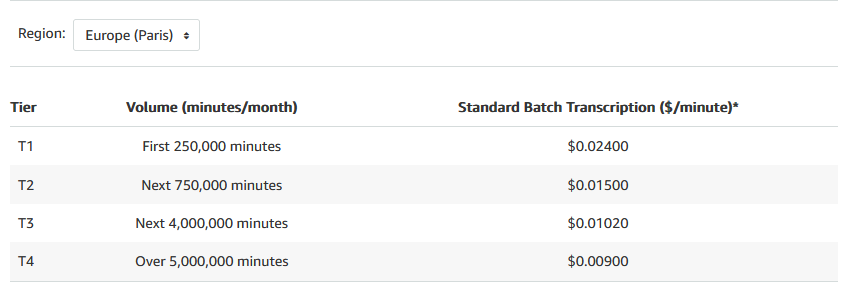
\includegraphics[width=\linewidth*3/4]{graphics/AmazonTranscribePricing.png}
    \caption{Prijzen Amazon Transcribe voor Parijse server \autocite{Amazon2023}}
    \label{fig:PricingAmazonTranscribe}
\end{figure}

\subsection{Microsoft Azure Speech Services}%

\paragraph{\IfLanguageName{dutch}{Beschrijving}{Description}}
Microsoft Azure Speech Services is een spraakherkenningsservice die wordt aangeboden door Microsoft Azure, het cloudplatform van Microsoft.

\paragraph{\IfLanguageName{dutch}{Functies}{Features}}
Azure Speech Services biedt een breed scala aan functies voor spraakherkenning en tekst-naar-spraak-conversie. Enkele van de belangrijkste functies zijn:

\begin{itemize}
    \item \textbf{Spraakherkenning}: De service kan gesproken taal detecteren en omzetten naar tekst in meer dan 60 talen. Het ondersteunt zowel real-time verwerking als batchverwerking van audiobestanden.

    \item \textbf{Taalherkenning}: Azure Speech Services kan automatisch de gesproken taal detecteren, waardoor het mogelijk is om meertalige spraakherkenning te realiseren zonder voorafgaande taalconfiguratie.

    \item \textbf{Aanpassing van modellen}: Gebruikers kunnen de spraakherkenning verbeteren en aanpassen aan specifieke vocabulaires en domeinen door aangepaste taalmodellen te maken. Hierdoor kunnen ze de nauwkeurigheid van de herkenning verhogen voor gespecialiseerde toepassingen.

    \item \textbf{Real-time streaming}: Azure Speech Services ondersteunt real-time streaming van spraak naar tekst, wat ideaal is voor toepassingen zoals live ondertiteling, spraakgestuurde opdrachten en interactieve dialoogsystemen.

    \item \textbf{Text-to-speech}: Naast spraakherkenning biedt de service ook mogelijkheden voor tekst-naar-spraak-conversie. Gebruikers kunnen tekst invoeren en de service genereert menselijke spraakuitvoer in verschillende stemmen en talen.
\end{itemize}

\paragraph{\IfLanguageName{dutch}{Tarieven}{Pricing}}
Per maand bied Azure vijf uur gratis aan daarna moet er een vergoeding van €0,935 betaald worden per uur.

\subsection{Mozilla DeepSpeech}%

\paragraph{\IfLanguageName{dutch}{Beschrijving}{Description}}
In tegenstelling tot de voorgaande services is DeepSpeech van Mozilla open source.

\paragraph{\IfLanguageName{dutch}{Functies}{Features}}
Mozilla DeepSpeech biedt verschillende functies en mogelijkheden voor spraakherkenning. Enkele van de belangrijkste kenmerken zijn:

\begin{itemize}
    \item \textbf{Hoge nauwkeurigheid:} DeepSpeech streeft naar hoge nauwkeurigheid in spraakherkenning en heeft aanzienlijke vooruitgang geboekt in termen van herkenningsscores.

    \item \textbf{Flexibiliteit:} Het systeem kan worden aangepast en afgestemd op specifieke toepassingen of vocabulaires. Hierdoor kan het worden gebruikt voor uiteenlopende spraakherkenningsscenario's.

    \item \textbf{Real-time verwerking:} DeepSpeech is ontworpen om spraak in realtime om te zetten, wat betekent dat het geschikt is voor toepassingen die onmiddellijke spraak-naar-tekstfunctionaliteit vereisen.

    \item \textbf{Privacy:} Als open-sourceproject stelt DeepSpeech gebruikers in staat om spraakherkenningssystemen lokaal uit te voeren, waardoor de privacy van gebruikersinformatie beter gewaarborgd is.
\end{itemize}

\paragraph{\IfLanguageName{dutch}{Tarieven}{Pricing}}
Aangezien dat de service open source is, moet er geen vast tarief betaald worden voor de service. Er kunnen echter wel kosten komen om de service te hosten.

\subsection{Whisper}%

\paragraph{\IfLanguageName{dutch}{Beschrijving}{Description}}
Whisper is de ASR service gemaakt door OpenAI. Het is beschikbaar als een API die ontwikkelaars kunnen integreren in hun eigen toepassingen en systemen door er spraakopnamen naar te sturen. De API geeft vervolgens een tekstuele weergave van de spraak terug als respons.

\paragraph{\IfLanguageName{dutch}{Functies}{Features}}
Whisper heeft verschillende kenmerken en mogelijkheden die het tot een krachtig spraakherkenningssysteem maken:

\begin{itemize}
    \item \textbf{Hoge nauwkeurigheid:} Whisper heeft aanzienlijke vooruitgang geboekt in termen van spraakherkenningsscores en streeft naar hoge nauwkeurigheid bij het omzetten van spraak naar tekst.

    \item \textbf{Meertaligheid:} Het model van Whisper ondersteunt meerdere talen, waardoor het geschikt is voor wereldwijde toepassingen en gebruikers met verschillende taalvereisten.

    \item \textbf{Flexibiliteit:} Whisper kan worden aangepast en afgestemd op specifieke toepassingen en vocabulaires, waardoor het kan worden gebruikt in uiteenlopende spraakherkenningsscenario's.

    \item \textbf{Real-time verwerking:} Het systeem is ontworpen om spraak in realtime te verwerken, wat betekent dat het geschikt is voor toepassingen die onmiddellijke spraak-naar-tekstfunctionaliteit vereisen.

    \item \textbf{Privacy:} OpenAI hanteert strenge beveiligings- en privacyrichtlijnen om de gebruikersgegevens te beschermen. Whisper stelt gebruikers in staat om spraakherkenningssystemen lokaal uit te voeren, waardoor de privacy van gebruikersinformatie beter gewaarborgd is.
\end{itemize}

\paragraph{\IfLanguageName{dutch}{Tarieven}{Pricing}}
Net als Mozilla's DeepSpeech is Whisper open source. Dit betekent dat de kosten afhangen van waar en hoe de service wordt gehost.

\subsection{Kaldi ASR}

\paragraph{\IfLanguageName{dutch}{Beschrijving}{Description}}
Kaldi ASR is een open-source spraakherkenningssysteem dat algemeen wordt gebruikt in de academische wereld en de industrie. Het is ontwikkeld door het Kaldi-project, een community-gedreven initiatief dat zich richt op het leveren van state-of-the-art spraaktechnologie.

Kaldi maakt gebruik van geavanceerde algoritmen en technieken, waaronder deep neural networks (DNN's) en hidden Markov models (HMM's), om spraak naar tekst om te zetten. Het biedt een flexibel en configureerbaar framework dat kan worden aangepast aan verschillende spraakherkenningstoepassingen.

\paragraph{\IfLanguageName{dutch}{Functies}{Features}}
Kaldi ASR biedt een breed scala aan functies en mogelijkheden die het tot een krachtig spraakherkenningssysteem maken:

\begin{itemize}
    \item \textbf{Hoge nauwkeurigheid:} Kaldi is bekend om zijn hoge nauwkeurigheid in spraakherkenning. Het maakt gebruik van geavanceerde modellen en trainingstechnieken om nauwkeurige resultaten te leveren.

    \item \textbf{Flexibiliteit:} Het Kaldi-framework is zeer configureerbaar en aanpasbaar. Het stelt gebruikers in staat om modellen en akoestische kenmerken aan te passen aan specifieke toepassingen en datasets.

    \item \textbf{Meertaligheid:} Kaldi ondersteunt meerdere talen en kan worden gebruikt voor spraakherkenning in verschillende taalomgevingen.

    \item \textbf{Uitgebreide toolkit:} Kaldi wordt geleverd met een uitgebreide toolkit die verschillende hulpmiddelen en utilities biedt voor spraakdataverwerking, modeltraining en evaluatie.

    \item \textbf{Community-ondersteuning:} Het Kaldi-project wordt ondersteund door een actieve gemeenschap van ontwikkelaars en onderzoekers, wat resulteert in regelmatige updates, bugfixes en nieuwe functies.
\end{itemize}

\paragraph{\IfLanguageName{dutch}{Gebruik en implementatie}{Usage and implementation}}
Kaldi ASR wordt meestal gebruikt via de command line-interface en vereist enige technische kennis om effectief te kunnen gebruiken. Het proces om Kaldi te gebruiken omvat het verzamelen en voorbereiden van spraakgegevens, het trainen van akoestische en taalmodellen, en het uitvoeren van de spraakherkenning op nieuwe gegevens.

Kaldi biedt documentatie en handleidingen om gebruikers te begeleiden bij de implementatie en het gebruik van het systeem. Het heeft een actieve gebruikersgemeenschap waar gebruikers vragen kunnen stellen en ervaringen kunnen delen.

\paragraph{\IfLanguageName{dutch}{Beschikbaarheid en prijs}{Availability and pricing}}
Kaldi ASR is een open-source project en is vrij beschikbaar voor iedereen. Het kan worden gedownload van de officiële Kaldi-website en lokaal worden uitgevoerd.


\section{\IfLanguageName{dutch}{Natuurlijke taalverwerking}{Natural Language Classifier}} \label{sec:Natural Language Classifier}%

\subsection{GPT series}%

\paragraph{\IfLanguageName{dutch}{Beschrijving}{Description}}
The GPT, wat staat voor Generative Pre-trained Transformer, series zijn algemene taalmodellen gemaakt door OpenAI. Het doel van deze modellen is genereren van menselijke taal op basis van de gegeven input. Het meest bekende voorbeeld is OpenAI's chatbot, ChatGPT. Het  maakt gebruik van GPT-3.5 en GPT-4 om antwoorden te genereren. Deze modellen zijn getraind op een brede set van internet data.

\paragraph{\IfLanguageName{dutch}{Tarieven}{Pricing}}
Er zijn twee GPT-4 modellen beschikbaar de 8K context en de 32K context. Om ze te gebruiken moet er betaald worden per 1000 tokens. Dat is ongeveer gelijk aan 750 woorden. Voor de 8K context is de prijs \$0.03 voor invoer en \$0.06 voor de uitvoer. De kost voor 32K context is \$0.06 voor invoer en \$0.12 voor het resultaat. Afhankelijk van het model is de prijs voor GPT-3 tussen de \$0.0004 of \$0.02 per 1000 tokens.

\subsection{BERT}%

\paragraph{\IfLanguageName{dutch}{Beschrijving}{Description}}
BERT, wat staat voor Bidirectional Encoder Representations from Transformers, is een ander type taalmodel ontwikkeld door Google AI Language. In tegenstelling tot de GPT-series, is BERT een bi-richtingstransformer, wat betekent dat het in staat is om zowel de context vóór als na een woord te begrijpen tijdens het trainen.

\paragraph{\IfLanguageName{dutch}{Tarieven}{Pricing}}
In tegenstelling tot de GPT reeks is BERT gratis te gebruiken. Het taalmodel vereist wel aanzienlijke rekenkracht en geheugen waardoor de hardware waarop het draait sterk genoeg moet zijn.

\subsection{FlairNLP}%

\paragraph{\IfLanguageName{dutch}{Beschrijving}{Description}}
FlairNLP is een NLP (Natural Language Processing) framework ontwikkeld door Zalando Research. Het staat voor "Flexible Language-Agnostic IRst-order" en is gericht op het bieden van flexibiliteit en veelzijdigheid in het verwerken van natuurlijke taal. Net als BERT en GPT maakt FlairNLP gebruik van transformer-gebaseerde modellen en kan worden gebruikt voor een breed scala aan taalverwerkings-taken.

\paragraph{\IfLanguageName{dutch}{Tarieven}{Pricing}}
Ook FlairNLP is open-source wat wil zeggen dat de kosten afhangen van hoe en waar de software op draait.

\subsection{RoBERTa}%

\paragraph{\IfLanguageName{dutch}{Beschrijving}{Description}}
RoBERTa staat voor "A Robustly Optimized BERT Pretraining Approach." Het is een door Meta AI ontwikkelde transformer-gebaseerd taalmodel en een doorontwikkeling van BERT. RoBERTa is ontworpen om de prestaties van BERT verder te verbeteren door middel van optimalisaties in de trainingsprocedure.

In tegenstelling tot BERT maakt RoBERTa gebruik van een grotere hoeveelheid trainingsdata en een langere trainingsduur, wat het model helpt om een dieper taalbegrip te ontwikkelen. Het trainingsproces van RoBERTa omvat het maskeren van woorden in een zin en het uitdagen van het model om de ontbrekende woorden correct te voorspellen, vergelijkbaar met BERT.

\paragraph{\IfLanguageName{dutch}{Tarieven}{Pricing}}
RoBERTa is net als BERT gratis te gebruiken.


%Dit hoofdstuk bevat je literatuurstudie. De inhoud gaat verder op de inleiding, maar zal het onderwerp van de bachelorproef *diepgaand* uitspitten. De bedoeling is dat de lezer na lezing van dit hoofdstuk helemaal op de hoogte is van de huidige stand van zaken (state-of-the-art) in het onderzoeksdomein. Iemand die niet vertrouwd is met het onderwerp, weet nu voldoende om de rest van het verhaal te kunnen volgen, zonder dat die er nog andere informatie moet over opzoeken \autocite{Pollefliet2011}.
%
%Je verwijst bij elke bewering die je doet, vakterm die je introduceert, enz.\ naar je bronnen. In \LaTeX{} kan dat met het commando \texttt{$\backslash${textcite\{\}}} of \texttt{$\backslash${autocite\{\}}}. Als argument van het commando geef je de ``sleutel'' van een ``record'' in een bibliografische databank in het Bib\LaTeX{}-formaat (een tekstbestand). Als je expliciet naar de auteur verwijst in de zin, gebruik je \texttt{$\backslash${}textcite\{\}}.
%Soms wil je de auteur niet expliciet vernoemen, dan gebruik je \texttt{$\backslash${}autocite\{\}}. In de volgende paragraaf een voorbeeld van elk.
%
%\textcite{Knuth1998} schreef een van de standaardwerken over sorteer- en zoekalgoritmen. Experten zijn het erover eens dat cloud computing een interessante opportuniteit vormen, zowel voor gebruikers als voor dienstverleners op vlak van informatietechnologie~\autocite{Creeger2009}.
%
%\lipsum[7-20]
